\chapter{TRASH (IN) ART}



\begin{singlespace}
\epigraph{One day, in a rubbish heap, I found an old bicycle seat lying beside a rusted handlebar, and my mind instantly linked them together. I assembled these two objects, which everyone then recognized as a bull’s head. The metamorphosis was accomplished, and I wish another metamorphosis would occur in the reverse sense. If my bull’s head were thrown in a junk heap, perhaps one day some boy would say, \quotes{Here’s something that would make a good handlebar for my bicycle!}}{\hfill ---Pablo Picasso, \textit{Trashformations}, 1998}
\end{singlespace}



This chapter questions the purpose and meaning of using trash as a medium in the artworks. Reasons and motivations of artists who use trash will be elaborated. Artists who use discarded items in their work will be analyzed in the light of arguments discussed in the previous chapter. Here, the main question is why artists select to use society's debris rather than fresh items. Hence, my research will focus on the place of trash in the world of art by looking at different methods and approaches. The scope of this research is started from masterpieces and founding works, and continued with recent examples of artworks.

Firstly I look at how artist started using objects that are not produced by herself/himself and with the purpose of making art. Considered early works are notable and founding ones that open new dimensions to reconsider objects and their meaning. Further, they extended the ways of art making and the language of art. Therefore, it is important and necessary to analyze them. In other words, I first look at the foundation of using non-art objects in the art making. Early examples are analyzed and how they evolved over time is explored. I try to find out how they affected successor artist. Secondly this chapter looks some examples of contemporary works. Particularly, I try to capture the current approaches on trash. Several methods and genres are explored. Lastly focused on the inspiring documentary of Agnès Varda, The Gleaners and I, which provides a general picture of the subject.



%****************************************
\section{Root in the Art History}
Using trashed objects in making art can be examined with the use of non-art objects in modern art. In other words, some artist started using objects in different scope beyond their intended purpose or intended meaning and function in their modern artworks. They develop their artworks by using paper and other stuff by pasting or juxtaposing them together.

From the beginning of 20th-century non-art objects draw attention of artists. Usage of these objects play significant role in the development of art trough time. Usage of these objects dramatically changed the way how people look at art. In short, they introduced a new way of making art.

One of the remarkable change in 20th-century art is the use of unconventional materials in the making of paintings and sculptures, rather than the conventional materials produced with the purpose of art. These objects are not commonly recognized as art often because they already have a non-art function. Their place in the society and people's mind commonly have a different meaning. Beyond that, artists started to use them for their own purposes. Thus, objects gained different meanings and usages with the hands of artists. It is explained in the previous chapter that objects are not static and absolute. Objects can be used for new purposes even if they lost their meaning and value in the conventional system.

Modern artist questioned the way of traditional way of art making in every dimension. Their approach is out of the previous methods. They are looking for the beyond of painting. With using different objects they break the pureness of artwork. It is not pure anymore, it is fragmented. They push the boundaries of art. Using non-art objects in the production of art challenges existing conventions of painting.

Using non-art object can be considered as moving away from the purification of art which is also significant movement in modern art. Purification argues the separation of art and the others. Abstract and minimalist works can be given as an example to the purification. However, methods such as collage and assemblage are a composition of different fragments and pieces. Rather than the traditional way of painting on canvas modern artists composed their work with the combination of various objects from different context. With this approach works can be examined in multi-dimensional context. This also represents another branch in modern art.

In 20th-century, modern artists experimented with new ways of seeing and with fresh ideas about the nature of materials and functions of art. Previously paintings are based on linear perspective and realistic style. Themes are often composed of religious and mythical narratives. After the second half of the 19th-century, they started to abandon these themes and painting methods. For instance, in the works of impressionist paint brushstrokes can be easily identified. In impressionist paintings, themes are composed of everyday scenes. With Cezanne, the linear perspective is started to question and later this questioning reached to its peak point with cubism. Cubism is developed with the collaboration of Picasso and Braque. Besides, these two artists experimented non-traditional materials in their works for the first time in the scope of fine art. They continuously produced works with using different objects. They support each others art. They showed that an endless potential lay there. They collaborated with each other on the development of cubism and collage. One of the keys to understand the significance of Cubism of Picasso and Braque, is to view their actions and how unusual they were for the time. When they placed mass produced artifacts into the realm of fine art they acted as artistic iconoclasts of their age.

Collage originates from the French \textit{coller} is a technique of pasting together manufactured, printed, or found materials, such as pieces of newspaper, fabric, wallpaper to a panel or canvas, frequently in combination with painting. In about 1912–13 Pablo Picasso and Georges Braque extended this technique, combining fragments of paper, oil-cloth, and newspapers with oil paint on canvas to construct compositions. Pasting paper is not a new technique but using this technique it in the art making is a revolutionary movement in the language of art \citep{waldman1992collage}. \quotes{Collage was a major turning point in the evolution of Cubism\footnote{It needs to be noted that there is two types of Cubism; analytical and synthetic. Analytical one early phase of cubism and based on fragmentary appearance of multiple viewpoints and overlapping planes. On the other hand synthetic one is the successor phase of analytical one and formed with various textures and patterns.}, and therefore a major turning point in the whole evolution of modernist art in this century} \citep{greenberg1984collage}.

Similar to the collage, assemblage is produced by the incorporation of three-dimensional objects. \cite{seitz1961art}, the curator of the exhibition \quotes{The Art of Assemblage} featured at the New York Museum of Modern Art in 1961, described assemblages as being made up of preformed natural or fabricated materials, objects, or fragments not designed as art materials.

One of the earliest and notable examples of collage is Picasso’s \textit{Still Life with Chair Caning} (Figure \ref{fig:Picasso_Chair}), in which a piece of oilcloth which is used as tablecloth or self coverings with an imitation chair caning design was pasted onto the painting. This work of Picasso also can be considered as first example of assemblage because of a rope that was used to frame the picture. Picasso combined painting with already existing materials. As mentioned in the name of the work, Picasso give clues of the parts of it. For instance the oval canvas and the rope around it represent the table. Pasted chair caning signifies the chair near the table. On the table folded paper shadow represent newspaper. Further there is a cut out lemon painted onto the table. The three letters above the scrap of cloth, \quotes{JOU}, can be understood as both the beginning of the word \quotes{JOURNAL}, referring to the customary newspaper lying across the cafe table, and as the French verb meaning \quotes{to play.} The new technique of collage provided new possibilities of playfulness. This was a new way of making art; instead of painting an object or landscape, you could paste whatever it was right onto the canvas.

\begin{figure}[h!]
  \centering
  \includegraphics[height=6cm]{graphics/picasso_chair.png}
  \caption{Pablo Picasso, \textit{Still Life with Chair Caning}, 1912, oil on oil-cloth over canvas edged with rope, 29 x 37 cm (Musée Picasso)}
  \label{fig:Picasso_Chair}
\end{figure}

Moreover, Braque and Picasso questioned the elitism of the art world, which had always dictated the separation of common, everyday experience from the contemplative realm of artistic creation. Of equal importance, their work highlighted and separated the role of technical skill from art-making. Braque and Picasso introduced a fake element on purpose, not to mislead or fool their audience, but rather to force a discussion of art and craft, of unique and mass-produced objects. They inquiry as \quotes{Can this object still be art if I don’t actually render its forms myself, if the quality of the art is no longer directly tied to my technical skills or level of craftsmanship?}

After Picasso and Baraque, many artists applied collage and assemblage techniques to their works. Dada artist Kurt Schwitters is one of the productive artists among them. In 1918 he created his own form of Dada in Germany named \textit{Merz}, using rubbish elements such as newspapers, bus tickets and pieces of broken wood in his collages and constructions. The nonsense word \textit{Merz} is generated from the name of a bank: the Kommerz und Privatbank. \textit{Merz} was soon to become a kind of brand name for almost all his productions. \cite{webster2011kurt} puts significance of Schwitters in the development of art as follows:

\begin{quote}
The language of \textit{Merz} now finds common acceptance and today there is scarcely an artist working with materials other than paint who does not refer to Schwitters in some way. In his bold and wide-ranging experiments he can be seen as the grandfather of Pop Art, Happenings, Concept Art, Fluxus, multimedia art and post-modernism...

Schwitters’ work inspired such post-war pioneers as Jasper Johns, Robert Rauschenberg and Joseph Beuys, and he is now seen as the grandfather of post-1945 art movements, from Pop Art to Fluxus, Conceptual Art to site-specific art, and the forerunner of present day artists such as Thomas Hirschhorn, Gregor Schneider and Rachel Whiteread.
\end{quote}

He is very insisted on what he did. He constructed his room sized construction \textit{Merzbau} several times in different locations. First one destroyed in the Second World War, the second by fire in 1951 and the only third one was preserved. They are never ending structures not static. Through his life he added bits and pieces to them. \cite{carroll2011ruin} explains art of Schwitters as follows:

\begin{quote}
The German avant-garde was working from ruins literally and metaphorically, and trash was both practically and freely available; to use it was an action that took the ruins of our society, its discarded, to question how meaning is constructed. Schwitters is able to use the ruined, the waste products, as an anthropological exploration of society from both its unpleasant outcomes and its decay. \ldots trash was both practically and freely available; to use it was an action that took the ruins of our society, its discarded, to question how meaning is constructed. As he wrote: \singlequotes{It grows more or less according to the principle of a metropolis.} The \textit{Merzbau} was itself a city; and just as Marx wrote that it was not the materiality of the object but the social relations that create value, the use of urban detritus in particular, the squalid results of mass-produced human relations, infuses the materiality of Schwitters’ work with an anthropological quality. Material has transformed into information, and \singlequotes{how} has surpassed \singlequotes{what} we see. The grottos in the \textit{Merzbau} that still reveal this detritus most clearly could not be re-created in Bissegger’s reconstruction because, arguably, they are an exploration of absence, an exploration of ruin.
\end{quote}

Jacknis \citep[as cited in][]{cerny1996recycled} claims that \quotes{like collage in art or quotation in literature, the recycled object carries a kind of \singlequotes{memory} of its prior existence. Recycling always implies a stance toward time ---between the past and the present--- and often a perspective on cultures ---one's own and others.}

Reused objects contain within them a reference to many separate times. Whatever their final design or destination, these reused non-art artifacts are, by definition, impure, inauthentic products of past and present, here and there, us and them \citep{cerny1996recycled}.

It is claimed that the end result is a category of hybrid objects that bear the mark of at least two distinct domains, each with its won material, meaning, makers, and users \citep{cerny1996recycled} Whatever their final function, each of these objects contains within itself a visual, material, and conceptual reference to multiple technologies, histories and places.

Collages and assemblages can be composed of all types of objects such as trash and found object. The notion of found object is researched by many scholars \cite{camic2010trashed, gascoyne1935short}, but usage in the art has gained new dimensions with the Duchamp's concept of ready-made. Industrially manufactured or anything found  anymore can found a place in the art. The most notable example is \textit{Fountain} (discussed in the previous chapter), a standard urinal purchased from a hardware store and displayed on a pedestal, resting on its side. Before that first one is \textit{Bicycle Wheel} (Figure \ref{fig:Duchamp_BicycleWheel}). He wrote that the idea of a bicycle wheel upside down onto a stool. Although he claimed to select objects for his ready-made without regard to beauty, he said, \quotes{To see that wheel turning was very soothing, very comforting\ldots I enjoyed looking at it, just as I enjoy looking at the flames dancing in a fireplace.} These samples were the beginning of 
shift from an art that is striving for beauty to a higher complex or hidden meaning beyond what was seen from common artifacts found in everyday living.

\begin{figure}[h!]
  \centering
  \includegraphics[height=6cm]{graphics/duchamp-bicycle-wheel-1913.jpg}
  \caption{Marcel Duchamp, \textit{Bicycle Wheel}, 1913 (authorised reproduction 1951)}
  \label{fig:Duchamp_BicycleWheel}
\end{figure}

% Found Object
Found object originates from the French \textit{objet trouvé}, describing art created from existing, but often modified, artifacts or products that are not commonly regarded as art, often because they already have a non-art function. They are generally picked up somewhere and their value for the finder might be aesthetic, symbolic and remembrance. \cite[170]{gascoyne1936short} by analyzing found objects in Surrealist art, writes that artist \quotes{discovers a hidden symbolic significance in the [found] object which is preserved when the object is \singlequotes{framed} as art.} In other words, the finder discovers an unrealised significance by removing found object from its previous context and placing it in a new one. The meaning of material artifacts was derived from their symbolic relation to another entities such as person, time, place, experience rather than through their physical attributes \citep{camic2010trashed}. \cite{camic2010trashed} notes that people's motivation and usage of found objects also occur in various ways. Further enjoyment through found objects is different than appreciating art in museums which is isolated and refined activity. On the other hand discoveries through found object might happen anywhere at anytime. Hence it is not boundaried activity and spread through the daily life.



%****************************************
\section{Examples from Contemporary Artists}
In the light of discussions at previous section, some of the main strategies and approaches of artist are analyzed here. In this section focus will be shifted to the examples from contemporary artists. First one is related with found objects

Photo booths are machines that place crowded places and with affordable cost people can get their photos. It is a phenomena that attract attention of artist and researchers such as Martin Parr and Gerry Badger who published history of them as two volume.

In the French film Amélie\footnote{Original title: Le fabuleux destin d'Amélie Poulain, in english: The Fabulous Destiny of Amélie Poulain} directed by Jean-Pierre Jeunet in 2001, young male character collects photos that are torn up and thrown away by their owner near photo booths spread through train and metro stations of Paris. He collects them and glue them together in a photo album. In the film photo booths and found photos are centrally catalytic. Amélie falls in love with him when she realize him searching for found photos. After his photo album passed to Amélie, she looks every page of photo album again and again. Through the images of unknown people, she establishes narratives that point out the significance of these images even if they are thrown away. The important part of the film, images of a man are generated who scavenge the photos of another people. There are a lot of artist who collects discarded items but their process is not well documented. Therefore we are not fully aware of their artistic process. 

\begin{figure}[h!]
  \centering
  \includegraphics[height=6cm]{graphics/amelie_01.jpg}
  \caption{Still image from Amélie by Jean-Pierre Jeunet}
  \label{fig:Amelie}
\end{figure}

Prior to film Amélie, British artist Dick Jewell published a book in title of \quotes{Found Photos} in 1977. It is a collection of photo booth images that had been thrown away or torn up by the people in the photos. \cite{walker2010dick} comments on that it is \quotes{always a joy to look through.} Images capture diverse range of activities and expressions of people using photo booth machine. They are scavenged by the artist from the photo booths of London. The reasons of why photos are rejected vary including technical problems like flash or posing time. On the other hand, some of them are very good condition, and it is a mystery that why they are rejected. Walker explains that the:

\begin{quote}
gap between our exterior perception of the image and what must have been the internal dissatisfaction of the original subject results in some of the effective moments in Found Photos, where the images are not only bizarre and wonderfully funny (as many of them are) but also profoundly moving.
\end{quote}

Walker argues that even if photo booths are mechanic and simple application of photography while capturing everyday life, leave behind such ambiguous and mysteries that some people trace them. \quotes{Dick Jewell’s approach with Found Photos was less interventionist, presenting the images themselves in the spirit of either an anthropologist showing his finds or a conceptual artist claiming bits of the real world as ready-mades.} His mode of discovery includes climbing to look at the top of the photo booths and looking for the nearest waste bin. Badger describes Found Photos as \quotes{both a conceptual artwork and a sociological footnote.}

\begin{figure}[h!]
  \centering
  \includegraphics[height=6cm]{graphics/DickJewell_FoundPhotos.jpg}
  \caption{Dick Jewell, \textit{Found Photos}, 1978}
  \label{fig:DickJewell_FoundPhotos}
\end{figure}

On the other side for another artist photographs serve a function to record his daily trash. Tim Gaudreau photographed every object that he threw away for one year. At the end around five thousand images are covered all the gallery and opened to visitors. He notes that it just started as a documentation of his discards, but later it became (part of his life and) an obsession that he can not able to easily quit off. He says that \quotes{this collection of images intimately displays what I do, what I consume. It reveals me.} Like in the case of Tracey Emin trash turns to a medium that is used to express oneself. People are not only composed of the listed items in the CVs, economical power like pointed out in the book (and also film) Fight Club Tyler Durden draws attention to the narrator by saying: \quotes{You are not your bank account.} It is an effective way of looking things left behind rather that things put forward. Through this project, artist reached better understanding what he is and notes that this project changed his consumption choices and patterns.

\begin{figure}[h!]
  \centering
  \includegraphics[height=6cm]{graphics/TimGaudreau_SelfPotraitRevealedByTrash.jpg}
  \caption{Tim Gaudreau, \textit{Self-Portrait as Revealed by Trash: 365 days of photographing everything I threw out – Variation I}, 2006, Photograph}
  \label{fig:TimGaudreau_SelfPotraitRevealedByTrash}
\end{figure}

Filomena Cruz turns her lens to the city and its trashes that are left behind, thrown away and squeezed on the sidewalk or pavement. In her photographic series \textit{Road Kill}, she captures tiny trash corpses that are generally ignored and out of sight. In other words, the skin of city revealed through her photos in micro scale. On the skin of city there are lots of trash including \quotes{a piece of chewing gum with an engraved leaf; a flattened-out tube; a corroding paper napkin with a still intact heart; or a frog-green Crayola melting in the heat, all speak the language of "worthlessness" suddenly becoming meaningful} as looked through the window of they capture the city life and skin of the city that we touched. She shows us tiny details of huge cities. Somehow these trashes for all effort succeeded to stay in the towns. These trashes can not be removed from the city but moved ones are stacked on landfill, and they are not tiny as they are.

\begin{figure}[h!]
  \centering
  \includegraphics[height=6cm]{graphics/FilomenaCruz_RoadKill_ReVista.jpg}
  \caption{Filomena Cruz, \textit{Road Kill}, 2014, Photograph}
  \label{fig:FilomenaCruz_RoadKill_ReVista}
\end{figure}

In the documentary film, Waste Land, Vik Muniz frames portraits of \textit{catadores} who are pickers of recyclable materials on the dump. He visits them at one of the biggest open-air garbage dump outside of the Rio de Janeiro home of the millions of people. Film documents whole process of development and production of "Pictures of Garbage" made of collected trash from dump. He selects unusual materials and people for portraits rather than the powerful and notable people as commonly encountered at Renaissance. To create portraits of \textit{catadores} there is any other material than trash because of they are already build up their life in trash of city. Also these images are sold an auction and earned money donated to the \textit{catadores}. The images of trash moved to beloved places such as homes and museums. As stated in the rubbish theory they transformed to a durable object.

\begin{figure}[h!]
  \centering
  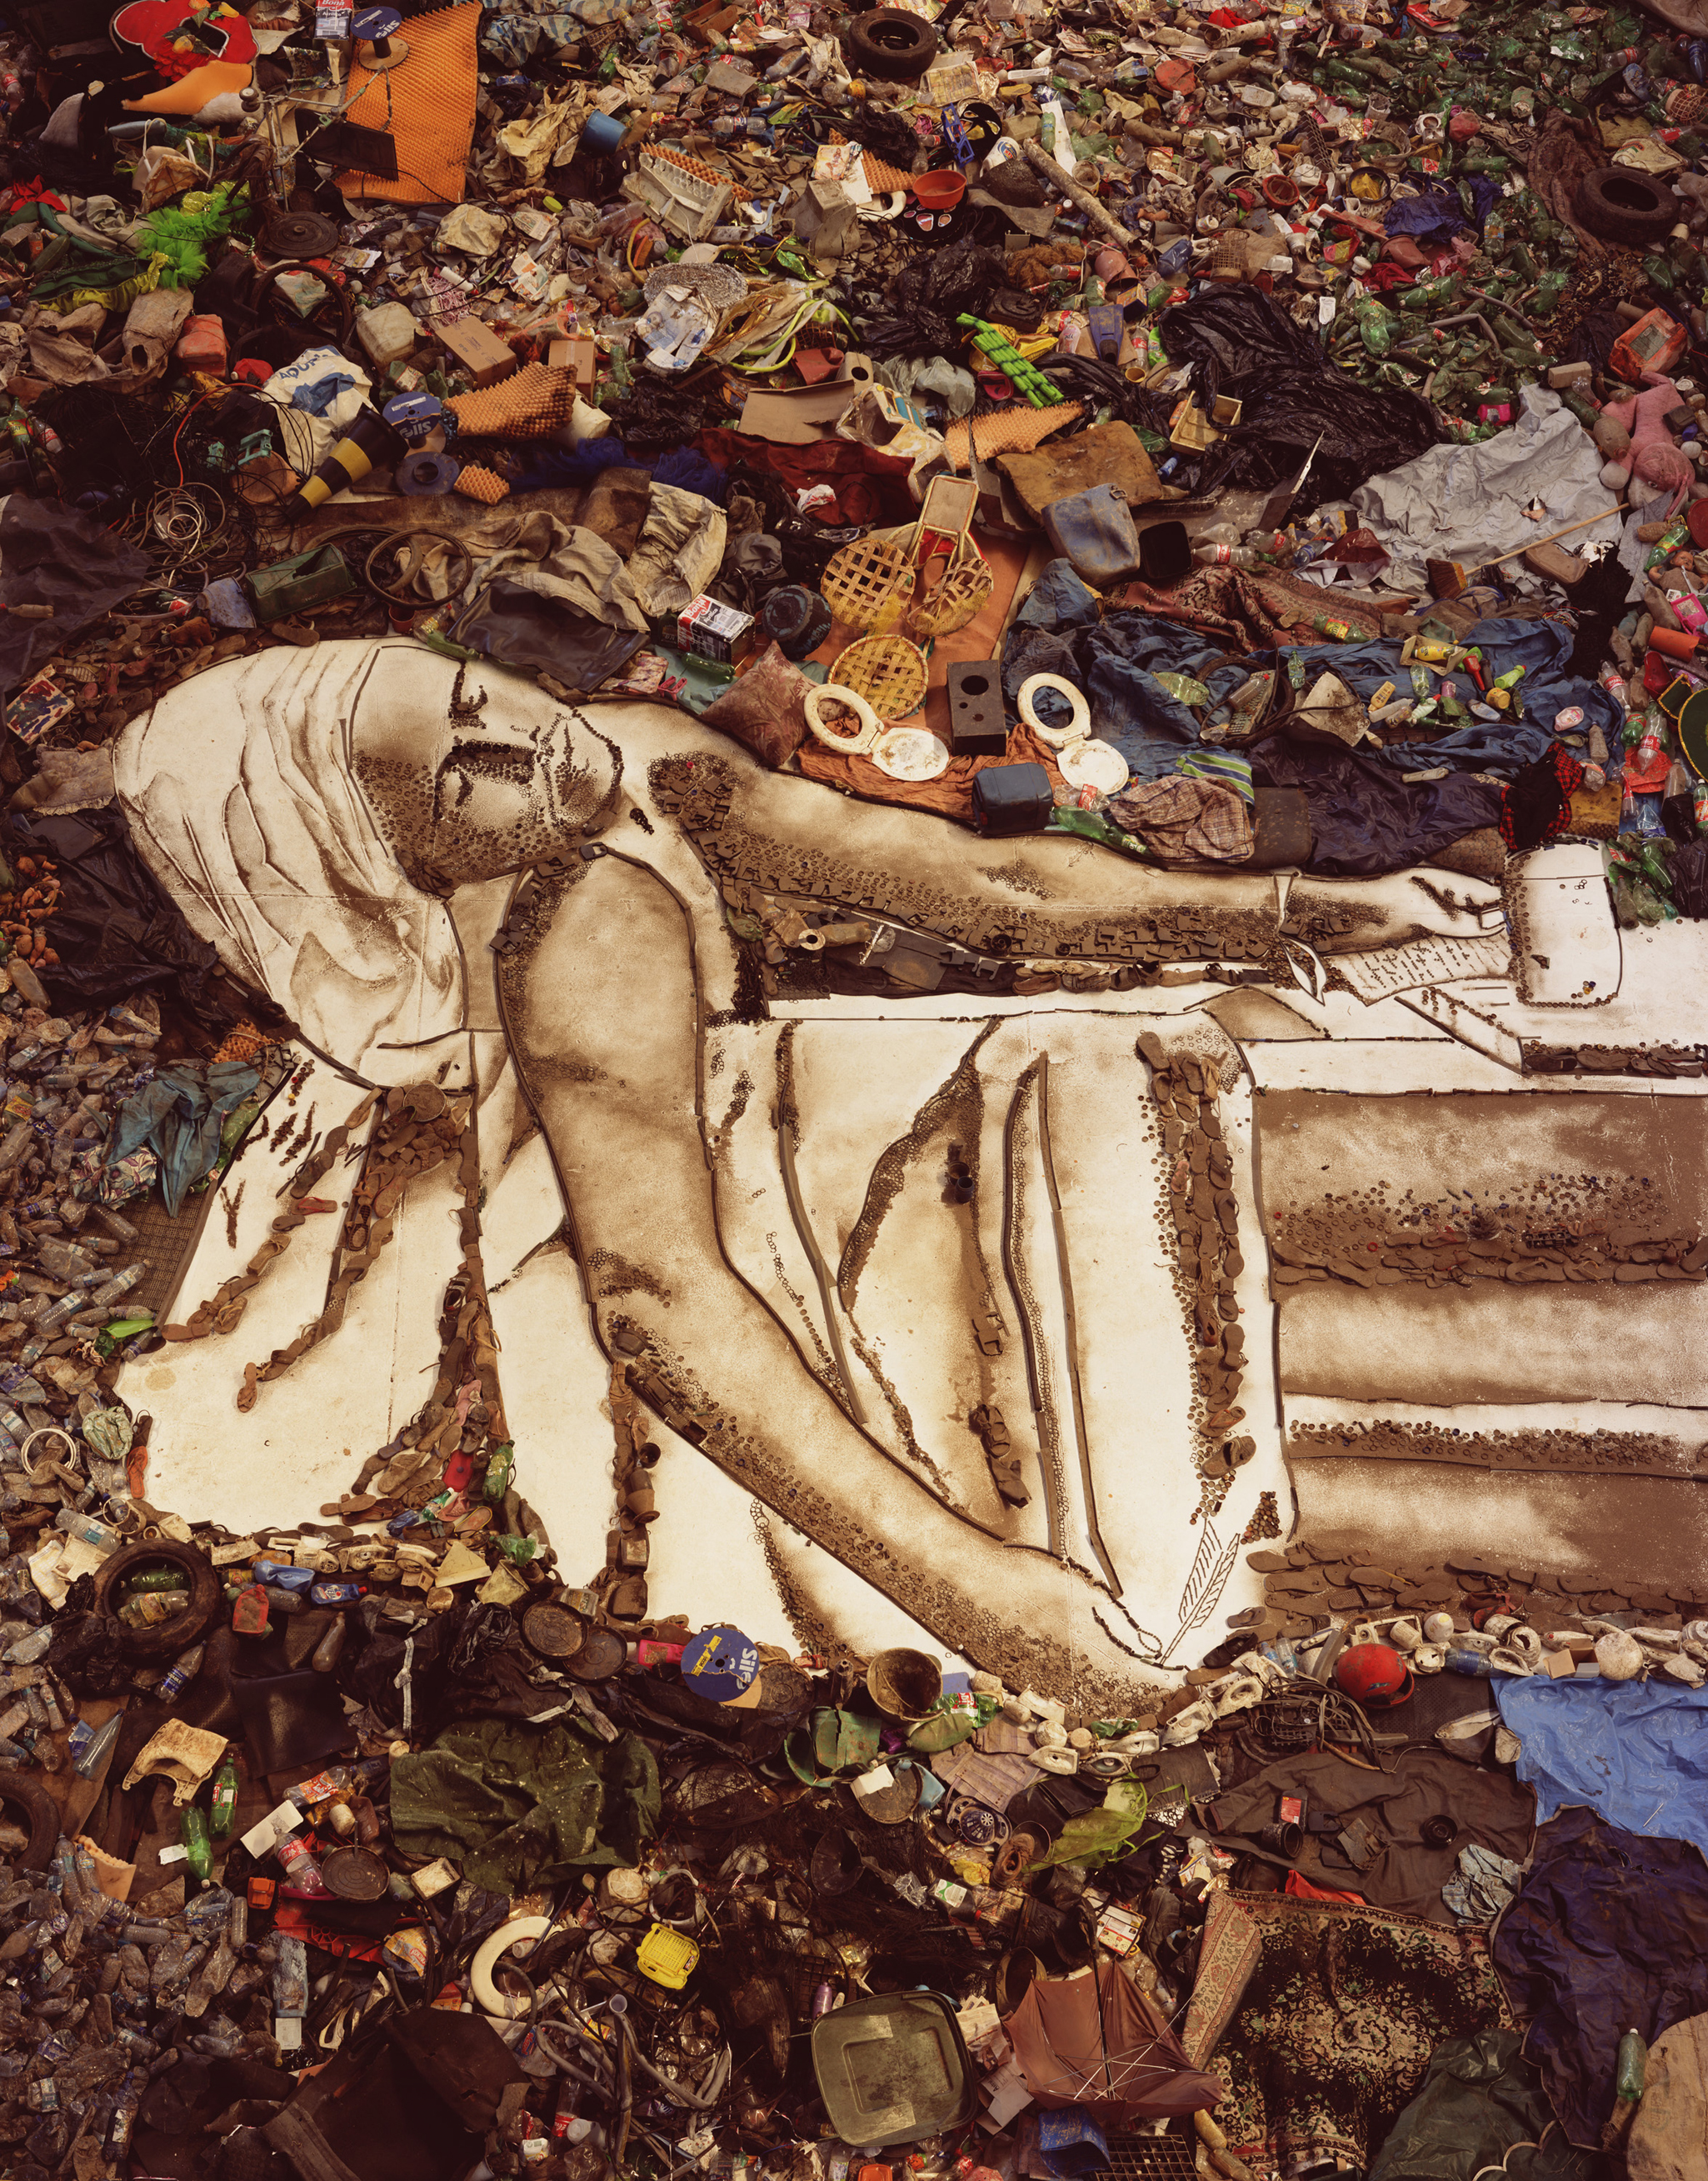
\includegraphics[height=10cm]{graphics/vik_muniz_marat.jpg}
  \caption{Vic Muniz, \textit{Marat}, 2008, mixed media, }
  \label{fig:VicMuniz_PicturesOfGarbage}
\end{figure}

Not only monumental portraits are extracted from the dump but also an orchestra is grounded up from the dump of Paraguay pioneered by Favio Chávez and Nicolás Gómez. Favio Chávez is a music teacher, and Nicolás Gómez is a garbage picker. They live in Cateura at Paraguay. It is a one of the poorest villages where people live among the sea of garbage. \quotes{A violin is worth more than a house here,} says Favio Chávez by pointing out their hard conditions. The orchestra's director and founder. Favio Chávez director and founder of the orchestra whose instruments such as violins, flutes and cellos are built from collected trash by Nicolás Gómez. Players of the orchestra are compiled from the children who are hopeless for their future. In the middle of such an existence, these people and musicians have created something both special and truly awe-inspiring. They are given birth to an orchestra that plays the masterpieces of classical music composed by Mozart, Beethoven, and Vivaldi. Trash turned to treasure and totally ironic that a signifier of high culture like classical music can be even played with imperfect instruments. For them and also, most of the people it is not affordable to buy an instrument and get the education of classical music. What they create is actually not expected from them, and their success is not limited with their location. They have given concerts around the world and their motto is: \quotes{The world send us garbage. We send back music.}

\begin{figure}
  \begin{subfigure}[b]{0.48\textwidth}
    \includegraphics[width=\textwidth]{graphics/landfill_harmonic-sax.jpg}
    \caption{Sax}
    \label{fig:landfill_harmonic-sax}
  \end{subfigure}
  \hfill
  \begin{subfigure}[b]{0.48\textwidth}
    \includegraphics[width=\textwidth]{graphics/landfill_harmonic-violin.jpg}
    \caption{Violin}
    \label{fig:landfill_harmonic-violin}
  \end{subfigure}
  \caption{Instruments of Recycled Orchestra}\label{fig:animals}
\end{figure}

As noted that recycling is an economic strategy of survival in developing countries throughout the world \citep[25]{cerny1996recycled}. Creative production that is motivated, primarily, by adverse conditions of economic necessity. Economic survival and adaptation are influential factors for both the makers, who build an informal business on the making and selling of recycled goods and the local consumers, for whom the market for affordable, utilitarian goods is devised. 

Nicolás Gómez builds musical instruments from what is available for him, in this case it is rubbish. His practice and works can be seen as an example of \textit{bricolage}. Dictionary meaning of it is something constructed by using whatever is available at hand. The French word \textit{bricoleur} is someone who works with own hands and construct \textit{bricolage}. The term coined by \cite[17]{levi1966savage} and he explains it as:

\begin{quote}
[He or she] is adept at performing a large number of diverse tasks; but, unlike the engineer, he [or she] does not subordinate each of them to the availability of raw materials and tools conceived and procured for the purpose of the project. His [or her] universe of instruments is closed and the rules of his [or her] game are always to make do with whatever is at hand, that is to say with a set of tools and materials which is always finite and is also heterogeneous because what it contains bears no relation to the current project, or indeed to any particular project, but is the contingent result of all the occasions there have been to renew or enrich the stock or to maintain it with the remains of previous construction or destruction. 
\end{quote}

In the scope of painting different than the works in the previous chapter (paintings on tea bags and coffee cups) historical portraits of notable people are painted onto the flattened aluminum drink cans which are disposable objects. The people in the figure \ref{fig:Alsbrooks} is General Jefferson C. Davis who was an officer at United States Army in 19th-century. Selected persons can be viewed as a member of the higher or ruling class of society. Therefore Kim Alsbrooks, painter of these works, might have thought that to make trash is more valuable, their face will be good or vice verse. She probably use trash to criticize social elite of that time. 

\begin{figure}[h!]
  \centering
  \includegraphics[height=8cm]{graphics/Alsbrooks.jpg}
  \caption{Kim Alsbrooks, \textit{Gen. Jefferson Davis}, 2015, oil on aluminum can}
  \label{fig:Alsbrooks}
\end{figure}

Not all the time and every artist turn trash into different objects, sometimes they only trash them. Michael Landy's Art Bin is one of them. It is a room size transparent bin placed inside of the art gallery. He invites people to bring their own artworks of failed attempts. Some of the notable contemporary artists such as Damien Hirst, Gillian Wearing, Tracey Emin and Mark Titchner participated in by throwing their sculptures, paintings, and prints into the Art Bin. People publicly toss their work from a high platform, and all of them can be seen outside of the transparent walls. He listens to the story and the failure of the artworks from their creator, and it is not allowed to throw others work. At one side he criticizes the idea of not aware of that artist also have lots of failures. People only can see the final work in the galleries and museums. In this work he break-ups this notion that encouraging the artist reveals their failures to the public. Like his words, it is “a monument to creative failure”. On the other side, there is a provocative approach to the art and art objects by saying that "Nothing is too good for the art bin." There is no limitation of throwing away even if art. 

\begin{figure}[h!]
  \centering
  \includegraphics[height=8cm]{graphics/MichaelLandy_ArtBin.jpg}
  \caption{Michael Landy, \textit{Art Bin}, 2014}
  \label{fig:MichaelLandy_ArtBin}
\end{figure}

Not all artist transform trash although some deconstruct them. Michael Landy is one of them. Michael Landy's Break Down Inventory is a two-week show (display) of destruction process of his all possessions on a dissemble line with the help of 10 workers. Firstly they are classified and recorded for three years and the deconstructed in two weeks by separating every element to the smallest part. Reveal all his possessions and deconstruct of them while he is alive. He turns them to rubbish and makes them unusable. Breaking down the all the meaning. Breaking down the connections. It can be an example of a downcycling process. It is preferred to decompose all the complex link and relationships between the objects. They are not just ordinary things they are possessions of the artist. Break Down 2001, in which he systematically destroyed all his personal possessions. His work examines what we value and what we discard, consumerism and waste, and human labor and its worth. It happens in public space. People can see the process. This process lasts two weeks at a place where people buy goods.

\begin{figure}[h!]
  \centering
  \includegraphics[height=7cm]{graphics/MichaelLandy_BreakDown.jpg}
  \caption{Michael Landy, \textit{Break Down}, 2001}
  \label{fig:MichaelLandy_BreakDown}
\end{figure}

The film American Beauty, which features a long, poetic clip of a plastic bag swirling on an eddy of air yet people find it hard to think of plastic bags as things of beauty. However, as a product --as something created and then unleashed to become seamlessly integrated into the lives of millions of people around the world--- there is a strange allure to them, just as a pathologist can admire the structure of a particularly virulent and contagious virus.

% TODO burayı da düzeltmek gerek.
Examples are not limited with these. Even if \quotes{trash is dirty and smelly trash can provide the raw materials for exquisite art---from sculpture to film and beyond.}



%
\section{The Documentary \quotes{The Gleaners and I} by Agnès Varda}
\quotes{The Gleaners and I} is a French documentary film directed by Agnès Varda in 2000. The film emphasizes diverse types of gleaning from rural to urban. According to the Merriam-Webster dictionary gleaning refers \quotes{to gather grain or other produce left by reapers}. Varda searches for the historical and current practices of gleaning in rural and urban areas of France. Historically, gleaning is the act of collecting what is left and not profitable crops after the harvest. By combining different fragments through his film, she shows that the act of gleaning also exists in various forms and styles. In particularly she curiously focuses on the (un)familiar people who glean leftover of society. Moreover, it is a self-reflexive film because the director establishes a relationship with the practice of gleaners and her film making practice. Some people glean crops; the others discarded food, and Varda gleans images.

The film is more than a research and document of the lives of many gleaners. It highlights the degree of global consumerism of the modern world and how technological advancements (or industrial (technical, modern) standards) result in waste. Varda seeks the several stages of potatoes from producers to consumers. As she discovers that supermarkets buy only potatoes that fit in industrial standards of shape and size. So what happens to the others? Varda discovers and shares with us the disturbing fact that they are taken back to the field where they came from, by following with the camera the trucks that unload mountains of potatoes. As Rosello notes that \quotes{The \singlequotes{good} potato is not the edible potato but one that will fit into a plastic container to be displayed on the shelf of a supermarket.} Varda records few people who glean the rejected potatoes from the field, and also she joins them by collecting heart shaped potatoes that fascinate her. Rosello explains that she is collecting not only refused potatoes but also images that are left behind.

\begin{figure}[h!]
  \centering
  \includegraphics[height=6cm]{graphics/AgnesVarda_Potatoes.jpg}
  \caption{Still image from The Gleaners and I}
  \label{fig:AgnesVarda_Potatoes}
\end{figure}

The industrial processes have some standards and beyond that standards, there is not a place for anything. It clears out (or move away) the rest. It can be viewed as the idealization of goods and products (even people). At this point, it can be referred back to Žižek's claim that people's false consciousness about balanced and idealized notion of nature. It can be understood that this type of clarification of objects may result in this false perception. What Varda's finding is an excellent exemplification of what Žižek wants to point out.

Contrary to the common act of discarding, Varda finds out a creative way to use her unconscious recorded piece that might be deleted by the others. It is the scene where Varda had forgotten to turn her camera off and accidentally films the ground and her lens cap bouncing along as she walks. She uses this scene with a jazz soundtrack at background. Watching this scene is confusing at first hand regarding context. It might be viewed as worthless and recorded by accident. One can ask that why is this placed here, what does this have to do with gleaning? However, Varda forces us to watch it (wants us to pay attention). This scene called as \quotes{the dance of the lens cap.} Ruth Cruickshank in the article, The Work of Art in the Age of Global Consumption: Agnes Varda’s \textit{Les Glaneurs et la glaneuse} (The Gleaners and I), addressed this scene and clarified the potential deeper meaning behind it. Cruickshank likened the scene to something that is normally thrown away, or in this case edited out of the film, much like the way trash is thrown away or food is left behind after a harvest. \quotes{Where many documentary makers would leave such accidental footage on the cutting room floor, Varda draws attention to how what would habitually be perceived as waste may be viewed as supplement with its own intrinsic value. Rather than literally treating it like dirt, Varda retains and prompts reassessment of that which is normally left out of shot} \cite{cruickshank2007work}. Things that are often forgotten or discarded can easily be revamped to create something useful to someone. The scene was revamped using music, and it became beautiful, much like the gleaners who found fish in the trash cooked it to make it edible, or the artist gleaner who piled discarded baby dolls into totem poles.

As Varda indicates, people can be found throughout the French countryside gleaning everything from apples to oysters, potatoes to grapes, much as they did hundreds of years ago (though no longer in organized groups). Making use out of something that has been left behind and labeled as obsolete is not unique to potatoes. There is so much discarded, yet still-viable food in dumpsters that many people live off it entirely. More metaphorically, there are also urban gleaners who scavenge scraps from bins, appliances from the side of the street, or vegetables from stalls after the markets have been closed. By showing them she explores that once was a common practice of gleaning throughout the years has evolved, but not disappeared. She keeps light to the modern life gleaners that are not visible every time. One of them is the teacher named Alain, an urban gleaner with a master's degree who teaches French to immigrants and refugees who are also considered as surplus of society. It can seen that from this example, gleaning becomes also a form of resistance to ruling system ---a way of rejecting to be limited by mainstream expectations and lifestyle.

She shows that the act of gleaning does not bound to the collecting food and survival reasons. Some of them build their own meaning, existence and identity through the collected items. One of the examples that she gave is that the man who collects baby dolls and use them in the decoration of his home. Every where is filled up with the baby dolls even if the wall of the garden.

Through the film she experiences the act of gleaning with different people. At one side she gleans potatoes in the field and on the other side follows a man with bicycle look for the garbage in front of the homes. By documenting their life in action she also participates their life. But she brings her own perception to them. For example in the case of potato gleaning she collects the heart shaped ones which attract attention of her. Moreover in the case of night searching, she finds a clock without hand. It has fulfilled its function and left away. Most important part of clock is missing therefore it is not functioning. However for her it has a different meaning. Not every time people seek to be aware of time sometimes they want to forget that.

A clock without hands found the garbage pile and taken by Agnès Varda. It does not work properly but it has important meaning for her. The time does not go on and it does not remind her that she is aging. One of the interesting thing is here Agnès Varda feels that as an aging person who will later become a discarded person.

Here another point is that Agnes records images of people picking up things from the ground like their ancestors. Everyone somehow collect things in their life but particularly she selects these people and their images in action. There should be a reason for this! For some individuals, gleaning is not a novelty or a clever way to save money, but a necessity of life. They require it to sustain their life. Combine the elements from different peoples that seems totally unrelated gains powerful theme for the documentary. What gleaning means become more open (or powerful). It draws a picture of body combination of different parts (connected, dependent to the each other). The reason of gleaning varies but the fact that gleaning is continues in different forms.

She discusses the importance of found in the meaning and purpose of art forms like this: \quotes{Varda seeks to encourage viewers to consider what potential agency is demonstrated in the artfulness and contingency of gleaning by individuals excluded\ldots from the homogenizing systems of global consumption} \cite{cruickshank2007work}. One can find more treasure in trash than many of New York’s finest galleries and art exhibits; they bring a grassroots feel to what has always been seen as a stuffy and prude aspect of society.

She investigates and talks artists who are using discarded items in their works. Which people could not find anything, the artists see countless possibilities. French collage artist Louis Pons is one of them. He specializes in reliefs and assemblages made wholly from refused materials and trash. Pons describes his artistic process and understanding of art as what others see \quotes{a cluster of junk,} he sees \quotes{a cluster of possibilities.} Varda records his studio which contains many scraps, pieces of junk with various shapes and color. Combination of these provide countless representations. By showing these people and their ideas about junk, Varda presents alternative ways to see objects and invites people to rethink. There is always alternative ways to see something different. It is like giving life or finding life from discarded object.







% TODO MOVE TO COMMON APPROACH, introduction.
%\comment{Semiotic Context, juxtapositions} \paraphrase{"In popular writing (such as novels), in television, films, music, and other forms of mass expression, the term trash is used to signify work that is of especially low value." \cite{lukas2012garbage}}



%%%
%%%
%%%
%\section{Summary}

% FROM drink UP, author: Werthan, Sarah, artist: Leech, Gwyneth. A Year in Cups. http://gwynethleech.com/
% trash and art collided. Paper and art, actually paper already medium of art, but is there anything different here. Itself is a part of a work, not the drawing, or painting.
% Documenting via a blog or a website. (what type of dimension it brings the work? maybe connect them, leave message.)
% Creating art in public places can demystify the process for passers by, Leech says, making artistic expression more accessible and part of people’s everyday lives. The reason of website.
% “People see that an artist can make work anywhere, and make creative spaces anywhere,” she asserts. 


% TODO PRAP. from rethink, reimagine, reinvent
%\paraphrase{Recycling art approach to using reclaimed objects in artworks requires rethinking, or examining the affordances of a particular object to explore the possibilities for the object's inclusion in an artwork. Assemblage art involves the creation of new and innovative objects from what were once considered objects of waste; that is. through their use in assemblage pieces, reclaimed objects are endowed with a new. sometimes paradoxical meaning. The transformations of the objects used in assemblage pieces ask viewers to reconsider the notion of "valuable" as they are challenged to look at everyday objects with a new perspective (Taylor, 2006). Viewers confront issues relating to the functionality of objects during modern processes of production, consumption and distribution.}





%"Garbage art (alternatively known as trash art or recycled art) is art created from materials including post-consumer and other waste, collected debris, or objects previously used for other purposes." "Creating art from garbage involves transforming the meaning of objects by placing them in new, aestheticized contexts. This practice is not new; tribal peoples have adapted bits of trash from industrialized societies into their traditional arts since coming into contact with products of the developed world." "Creating art from trash involves “consuming” garbage in the sense that artists appropriate and rearrange the materials in personal ways, transform their meanings, utilize them to their own ends, and represent them in new ways.It involves taking unwanted materials out of their “waste” context and recontextualizing them as “art.”" \cite{tauxe2012encyclopedia}





%
%
%\textbf{What might be the meaning of using trash as a medium in the artworks? Questioning trash as a medium for artist}
%\begin{itemize}
%\item Some works try to raise awareness the problems that are the result of trash. (It treats environment and nature.)
%\item Some of them reflect people's lifestyle especially throw away culture. As a mirror of current lifestyle.
%\item Try to find a new value and meaning from the discarded material that are useless anymore. To explore a new approach, new way. Subvert people's ideas about trash and their attitudes by turning materials to the something meaningful (or valuable). Trash to treasure.
%\item Using discarded item to represent other discarded things by the ruling ideology or approach. For example, trash can be used to represent refugees. The things that we are trying to discard does not mean that they have no value, instead it means that we have no ability to reveal its potential. In other words, refugees have potential but we see them as players that will change our current system. Therefore, it can be said that willing to transform trash to treasure is to require change of current lifestyle. Rejecting discarding something especially thing that you get value from it is a process and spread through to the ones life.
%\item One way is not to produce trash. (Zero trash philosophy.) The other one is to transform trash into something else.
%\item What type of experience is that collecting and working on objects that are generally discarded? Experiencing out of common practice, being open to new explorations.
%\item Instead of a world that produce trash, how could it be a world created from trash?
%\item Combining industrial goods with objects transformed from trash is another way to find a place to trash in the community. It also signifies that trash still has a good quality to used with new materials. Creating composite products from new and reused items. Using the valuable thing with the invaluable thing. It becomes more valuable or less valuable. Depends on the perception.
%\item Aesthetics of trash. Revealing aesthetics value of discarded stuff. (Unique visual value. Trash portraits, sculptures etc.)
%\end{itemize}




% TODO From Beautiful Trash Art and Transformation BY PAOLA IBARRA, ReVista
%Recycling has always been a common practice in the arts at least at a non-material level. From creating a world of words in literature, to rhythm and images in poetry, sampling in hip hop music, representation in the visual arts, or editing the illusory continuity of a film, art implies taking disparate elements (ideas, images, references, objects, etc.) and putting them together to form a new whole. Take and put. De-contextualize and re-contextualize. In that sense, art, as a system, is an act of recycling [from PAOLA IBARRA]. 

% TODO new comer
% FROM Book: Recycled, Re-Seen: Folk Art from the Global Scrap Heap
%\summary{Resistance} 
%\comment{Resistance, tactile, agnes varda?} If it is ultimately romantic to speak of these toys (or any other modern-day recyclia) in the language of resistance (by which I mean self-conscious political opposition), I would agree with Marshal Sahlins's assertion that "whether or not it comes to this [resistance], the indigenous mode of response to imperialism is always culturally subversive, insofar as the people must need to interpret the experience and they can do so only according to their own principles of existence. (sahlins 1992, 16)"

% TODO new comer
% FROM Book: Recycled, Re-Seen: Folk Art from the Global Scrap Heap
%\summary{Ironic}
%\comment{IRONIC, maybe added to results of transformation, reusing trashed items in different contexts.} This misuse the detritus of the industrial age has been described by western theorist as ironic. the irony is often embodied visually and conceptually. opposite of natural use, expected perception. for example making something from nothing or turning trash into treasure. By juxtaposing different materials changing context and place. 
